Proses desain mekanik dari robot hexapod ini meliputi tiga bagian utama, yaitu
desain kaki robot, desain rangka robot, dan desain lengan serta kepala robot.
Selurh bagian dirancang menggunakan perangkan lunak \emph{SolidWorks}. Pengguaan \emph{SolidWorks}
didasari dengan tujuan untuk mendapatkan model tiga dimensi yang dapat dianalisa lebih lanjut
dan untuk mempermudah proses pembuatan robot hexapod ini.
\begin{figure} [H] \centering
  % Nama dari file gambar yang diinputkan
  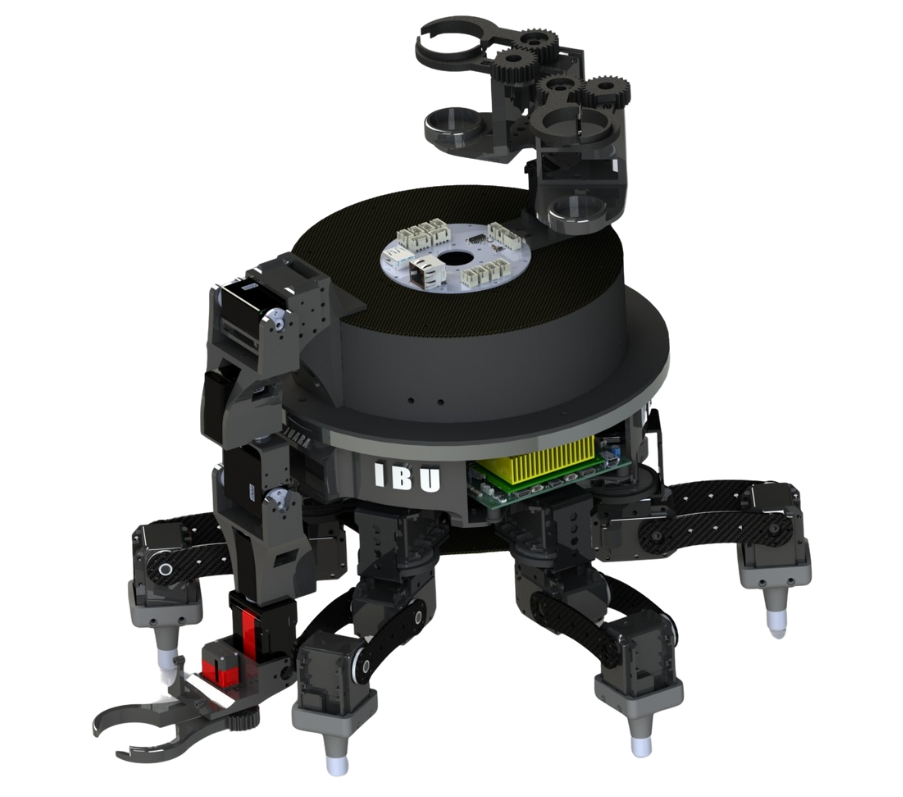
\includegraphics[scale=0.35]{gambar/Phynix2.png}
  % Keterangan gambar yang diinputkan
  \caption{Desain 3D Robot Hexapod}
  % Label referensi dari gambar yang diinputkan
  \label{fig:PHYNIX2}
\end{figure}

\subsection{Desain Base Kaki Robot} Proses desain base kaki robot meliputi
proses pembuatan desain tiga dimensi dari kaki robot dan base robot. Setiap kaki
robot memiliki tiga buah \emph{joint} yang masing-masing dihubungkan dengan
\emph{link} yang berfungsi sebagai penghubung antar \emph{joint} seperti pada
gambar \ref{fig:base_samping}. Bagian base robot berfungsi sebagai tempat pemasangan kaki robot dan
tempat \emph{power board}. 
\begin{figure} [H] \centering
  % Nama dari file gambar yang diinputkan
  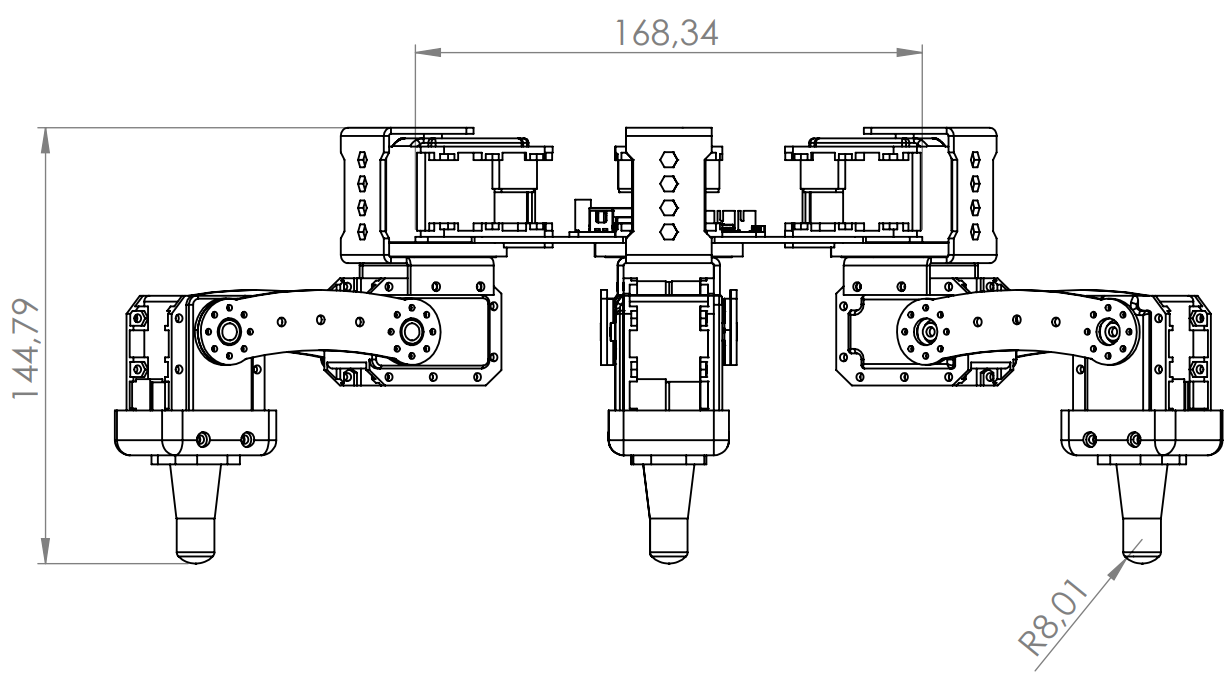
\includegraphics[scale=0.4]{gambar/base_kaki_samping.png}
  % Keterangan gambar yang diinputkan
  \caption{Base Tampak Samping}
  % Label referensi dari gambar yang diinputkan
  \label{fig:base_samping}
\end{figure}

\begin{figure} [H] \centering
  % Nama dari file gambar yang diinputkan
  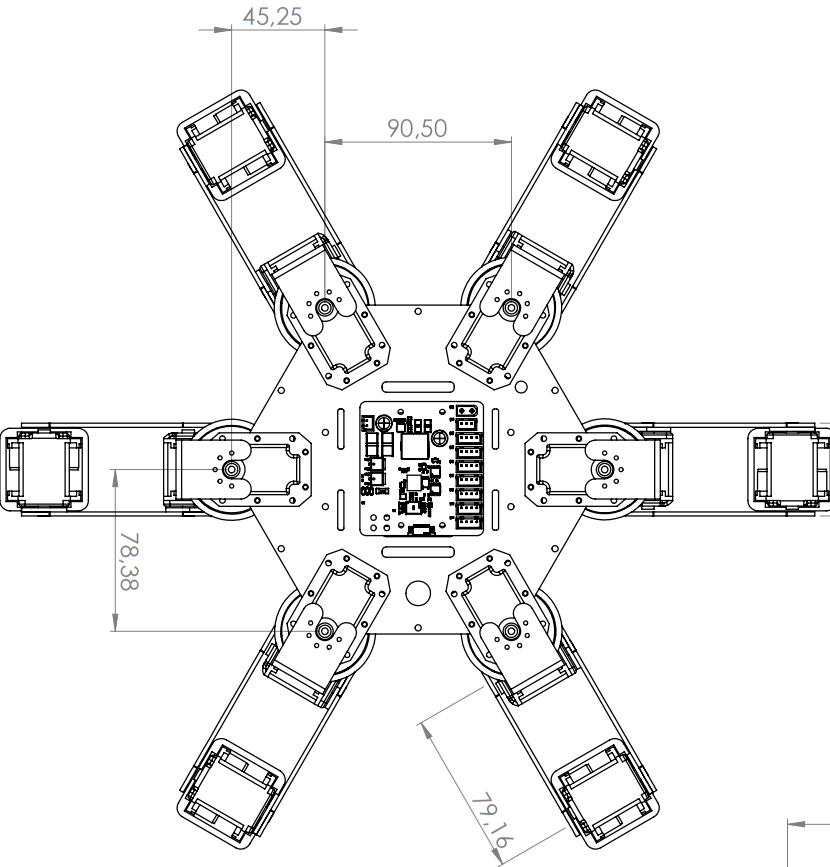
\includegraphics[scale=0.4]{gambar/base_kaki_tengah.png}
  % Keterangan gambar yang diinputkan
  \caption{Base Tampak Atas}
  % Label referensi dari gambar yang diinputkan
  \label{fig:base_atas}
\end{figure}

\subsection{Desain Rangka Utama Robot}
Rangka utama robot merupakan bagian yang menghubungkan antara base
kaki dengan kepala robot. Rangka utama robot menjadi tempat untuk 
meletakkan \emph{main board}, baterai 4 sel, dan baterai 2 sel. 
Bagian atas dari rangka utama robot terdapat sebuah slip ring 
yang berfungsi untuk menghubungkan kabel pada kepala robot
dengan kabel pada rangka utama robot tanpa perlu khawatir kabel
terpuntir ketika kepala robot berputar. Bagian slip ring akan diputar
dengan sebuah motor servo yang dipasang pada rangka utama robot. 
\begin{figure} [H] \centering
  % Nama dari file gambar yang diinputkan
  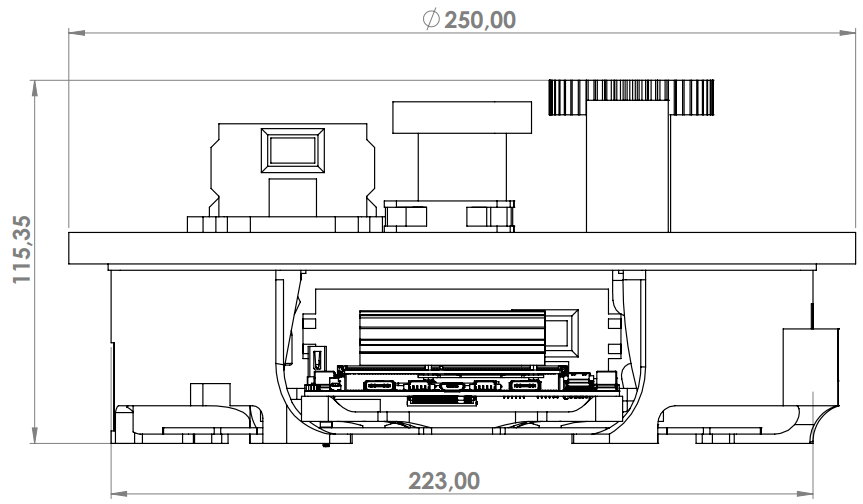
\includegraphics[scale=0.4]{gambar/rangka_utama_samping.png}
  % Keterangan gambar yang diinputkan
  \caption{Rangka Utama Tampak Samping}
  % Label referensi dari gambar yang diinputkan
  \label{fig:rangka_utama_samping}
\end{figure}

\begin{figure} [H] \centering
  % Nama dari file gambar yang diinputkan
  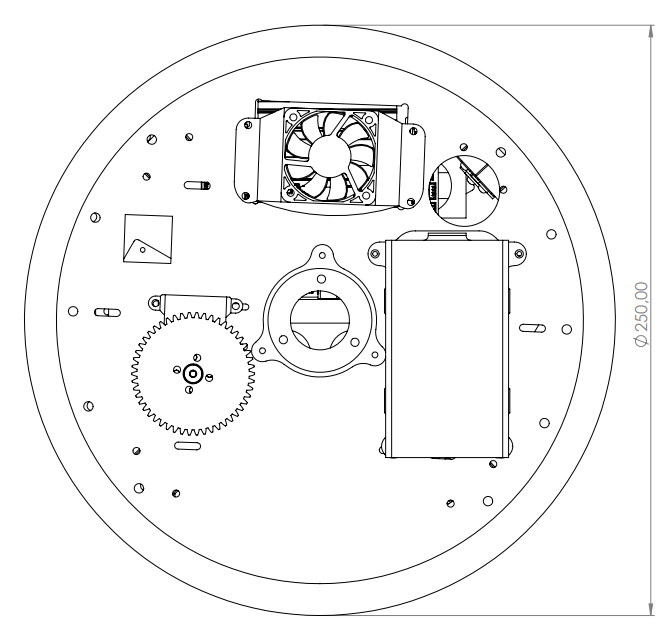
\includegraphics[scale=0.4]{gambar/rangka_utama_atas.png}
  % Keterangan gambar yang diinputkan
  \caption{Rangka Utama Tampak Atas}
  % Label referensi dari gambar yang diinputkan
  \label{fig:rangka_utama_atas}
\end{figure}

\subsection{Desain Kepala Robot}
Bagian kepala robot merupakan bagian yang menempel pada rangka utama robot. Bagian kepala dapat berputar 
sebesar 360$^{\circ}$ secara terus-menerus dengan bantuan motor servo pada
rangka utama robot. Sisi bagian depan kepala robot menjadi tempat lengan
robot 6-DOF, Seberang dari lengan robot menjadi tempat untuk dua buah
gripper yang berfungsi sebagai tempat penyimpan objek yang diambil
oleh lengan robot.   
\begin{figure} [H] \centering
  % Nama dari file gambar yang diinputkan
  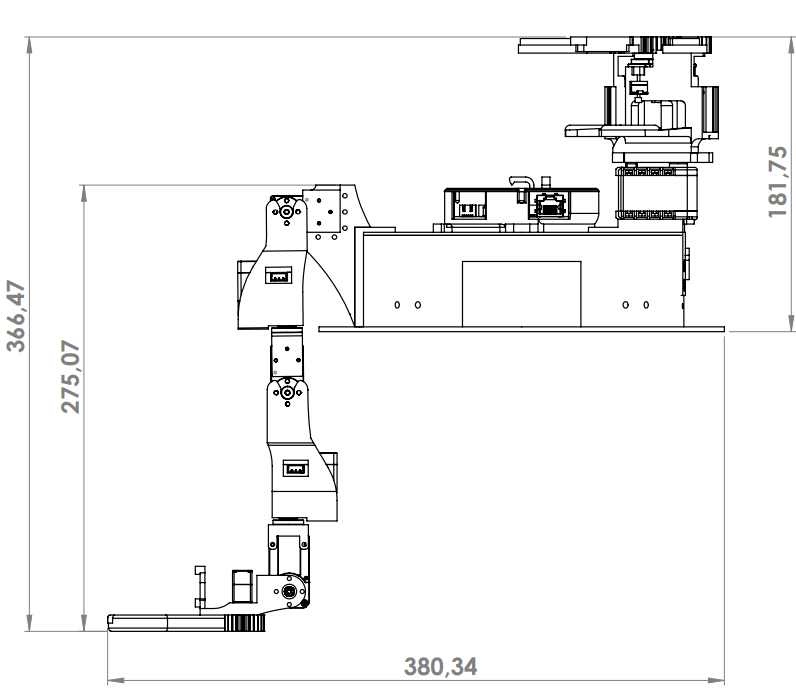
\includegraphics[scale=0.4]{gambar/kepala_samping.png}
  % Keterangan gambar yang diinputkan
  \caption{Kepala Robot Tampak Samping}
  % Label referensi dari gambar yang diinputkan
  \label{fig:kepala_samping}
\end{figure}

\begin{figure} [H] \centering
  % Nama dari file gambar yang diinputkan
  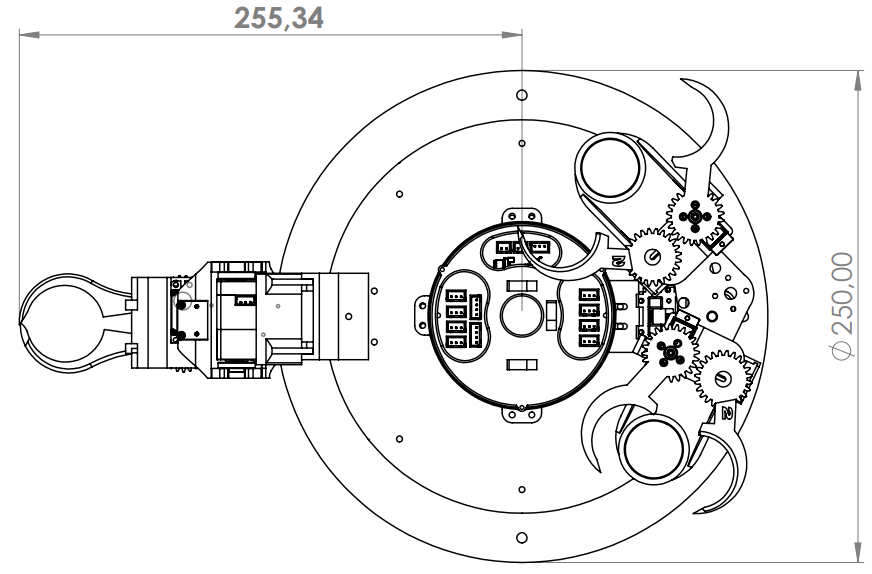
\includegraphics[scale=0.4]{gambar/kepala_atas.png}
  % Keterangan gambar yang diinputkan
  \caption{Kepala Robot Tampak Atas}
  % Label referensi dari gambar yang diinputkan
  \label{fig:kepala_atas}
\end{figure}
